\documentclass[a4paper,12pt,twocolumn]{article}
\usepackage[czech]{babel}
\usepackage[left=1.5cm,text={18cm, 25cm},top=2.5cm]{geometry}
\usepackage[IL2]{fontenc}
\usepackage[utf8]{inputenc}
\usepackage{svg, amsmath, amsthm, amssymb}
\usepackage{times}

\begin{document}
\begin{titlepage}
  \begin{center}
	
\includegraphics[origin=c,scale=0.5]{fit}
	\\[60mm]
    {\Huge Signály a systémy}\\[5mm]
	{\Huge Protokol k projektu}\\[5mm]
    \vspace{\stretch{0.618}}
    \Large{2018}\hfill Matej Soroka (xsorok02)
  \end{center}
\end{titlepage}

\section{}
Vzorkovacia frekvencia signálu: 16000Hz\\
Dĺžka vo vzorkoch: 32000\\
Dĺžka v sekundách: 2\\
Počet reprezentovaných binárnych symbolov: 2000
\section{}
Signál preiterujem, s tým rozdielom že sa na začiatku posuniem o 8 vzoriek, a následne sa posuvám o 16 vzoriek po každej iterácii. V každej iterácii taktiež vyhodnocujem binárnu hodnotu podľa hodnoty signálu v danom bode a ukladám ju do poľa.
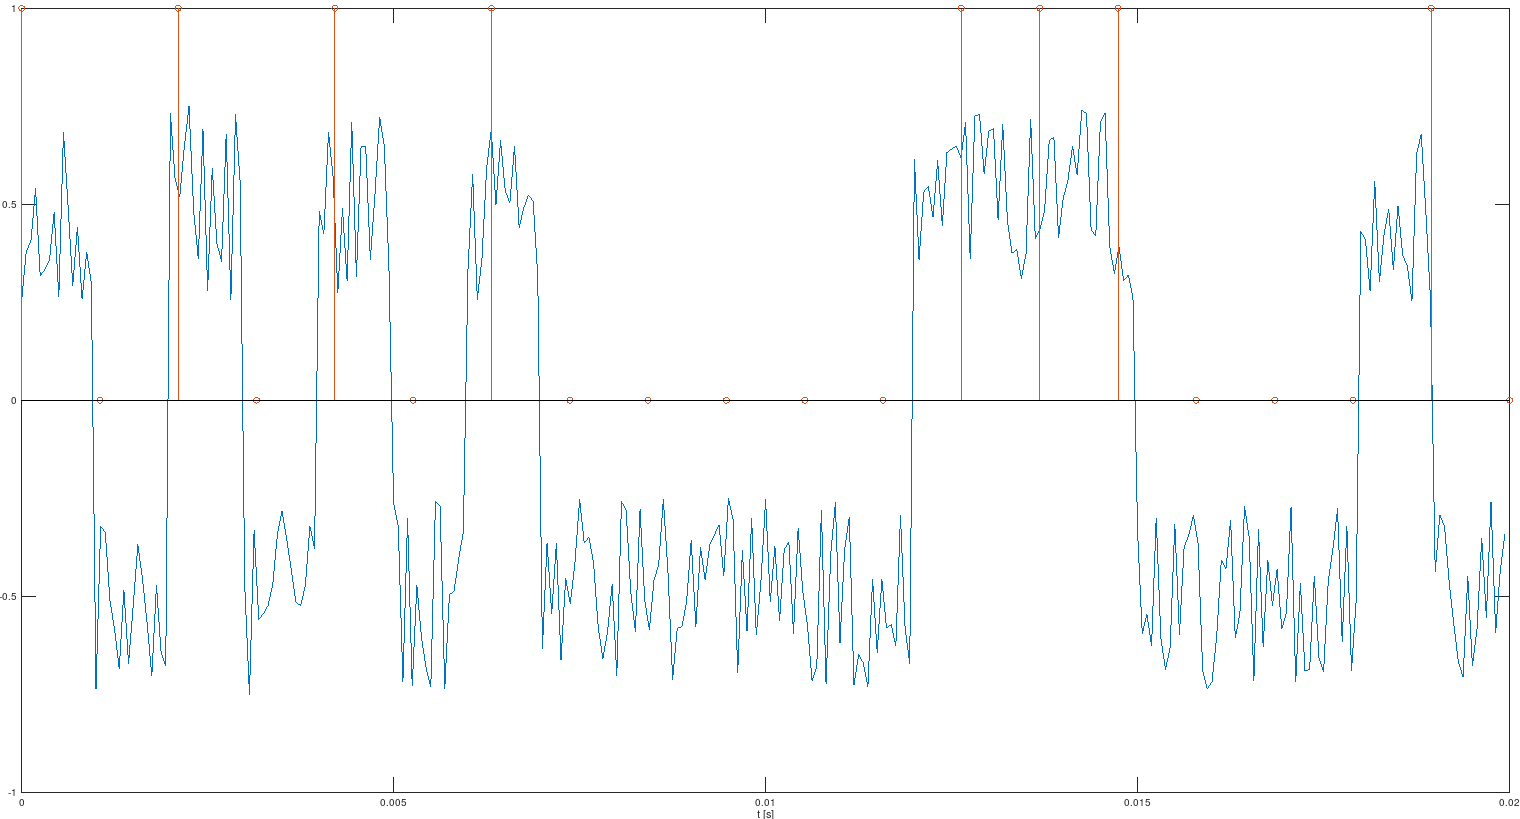
\includegraphics[width=\linewidth]{2}
\section{}
Filter je \textbf{stabilný}, všetky póly sú vo vnútri jednotkovej kružnice, platí vzťah $ |p_k| < 1 $.
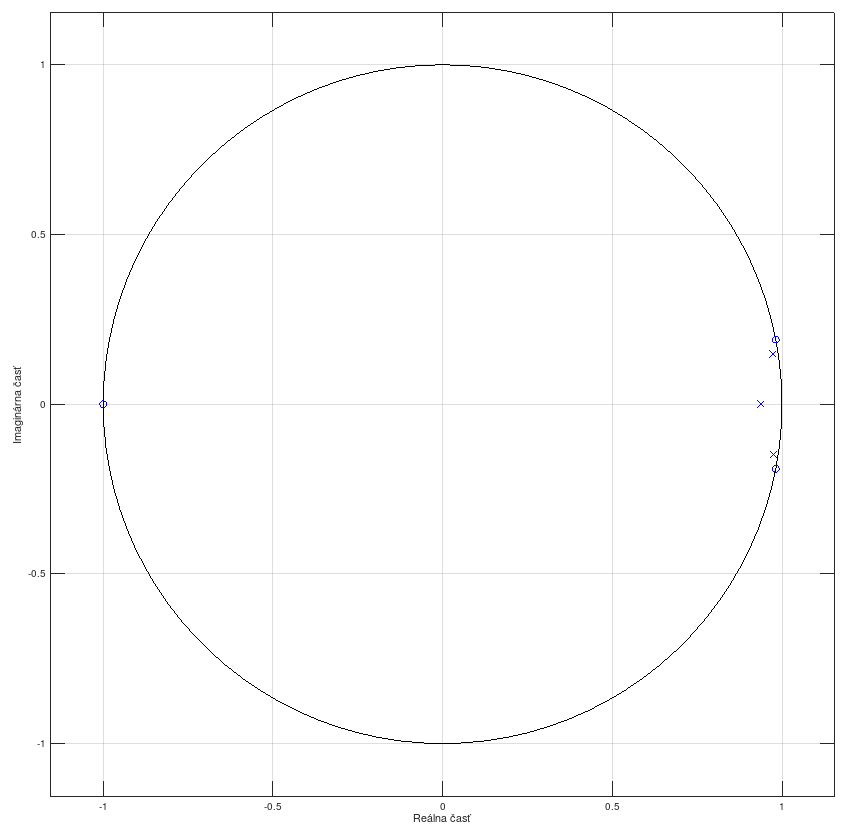
\includegraphics[width=\linewidth]{3}
\section{}
Filter je typu dolná priepusť, ako vidíme v grafe. Medzná frekvencia je 487.25Hz.
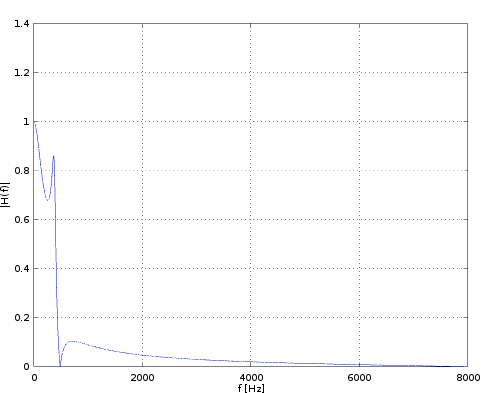
\includegraphics[width=\linewidth]{4}
\section{}
Využil som oneskorenie o 15 vzorkov. Snažil som sa o pretnutie osi x približne v čase 0.012s
\section{}
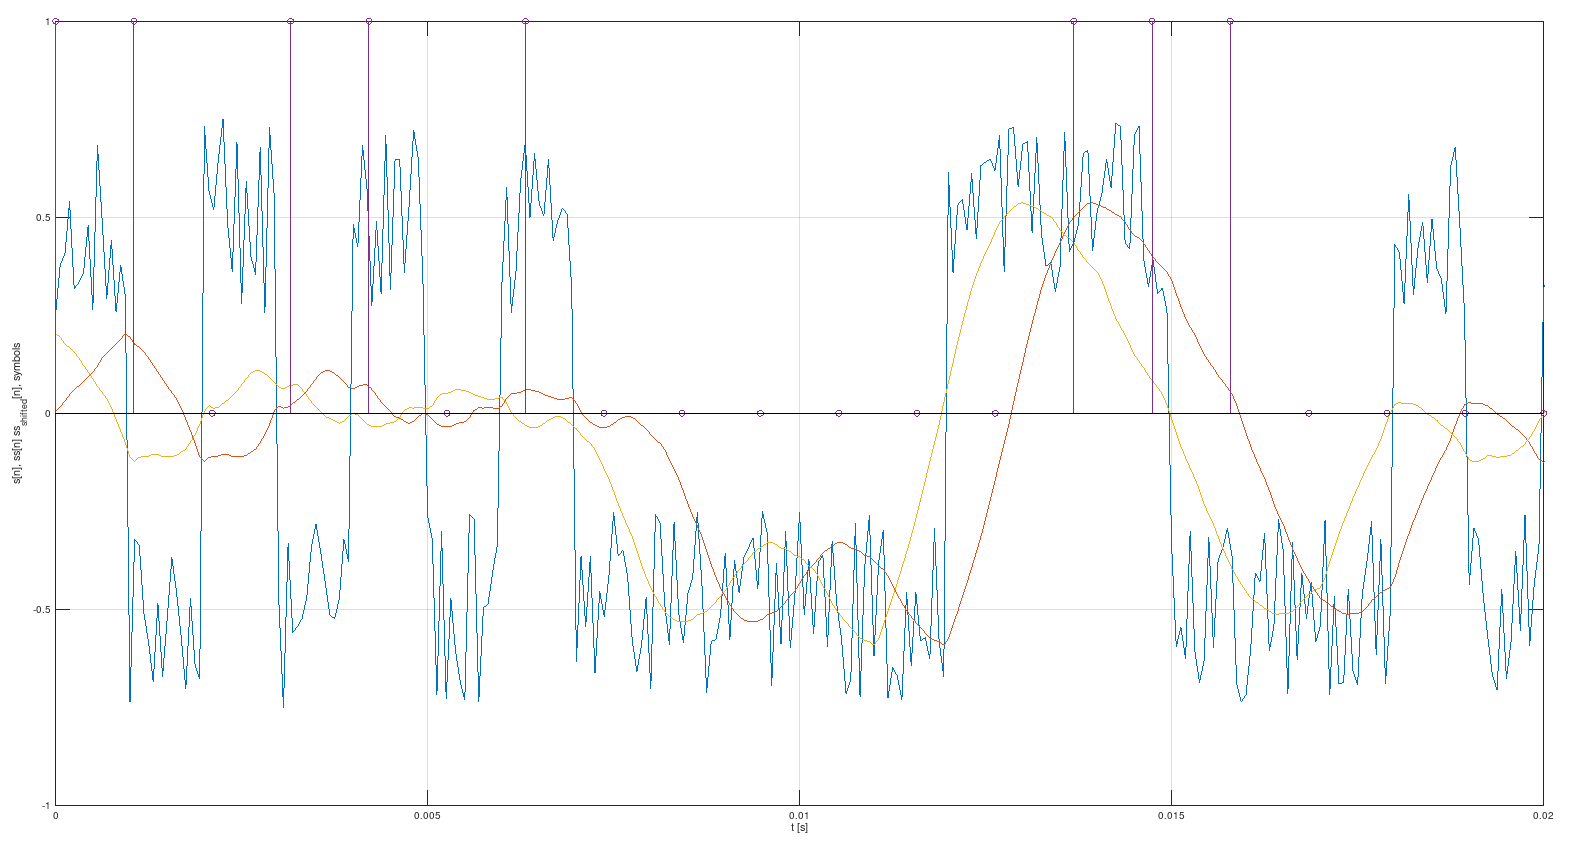
\includegraphics[width=\linewidth]{6}
\section{}
Kedže som signál posunul o viac ako 8 vzoriek, využil som o jednu vzorku menej.\\
Počet chýb: 1999\\
Celkový počet vzorkov: 83\\
Chybovosť: 4.1521\%
\section{}
% TODO: ??? komentovat ako vyzeraju signaly
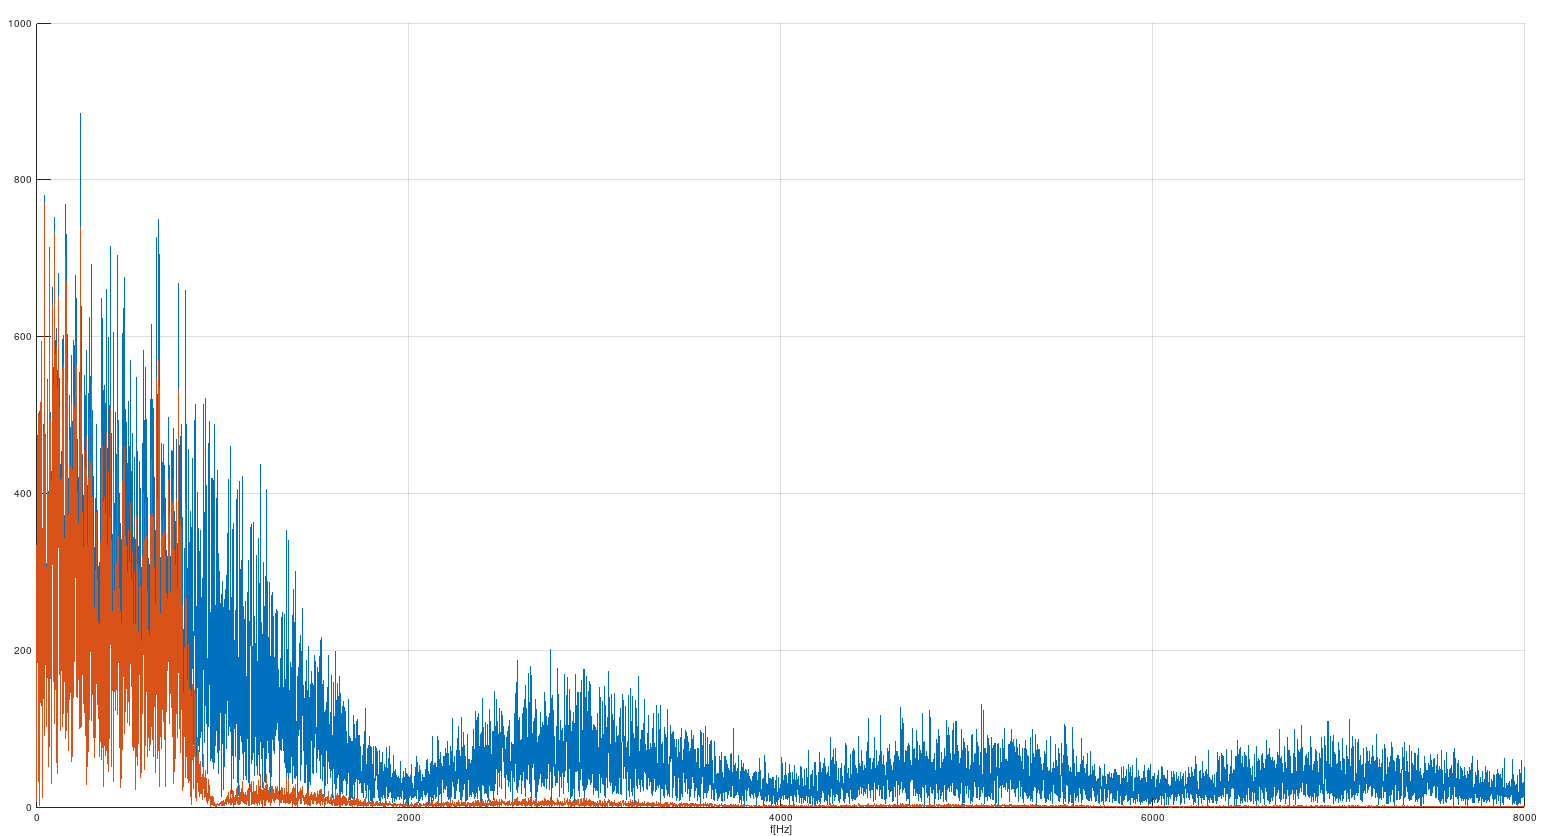
\includegraphics[width=\linewidth]{8}
\section{}
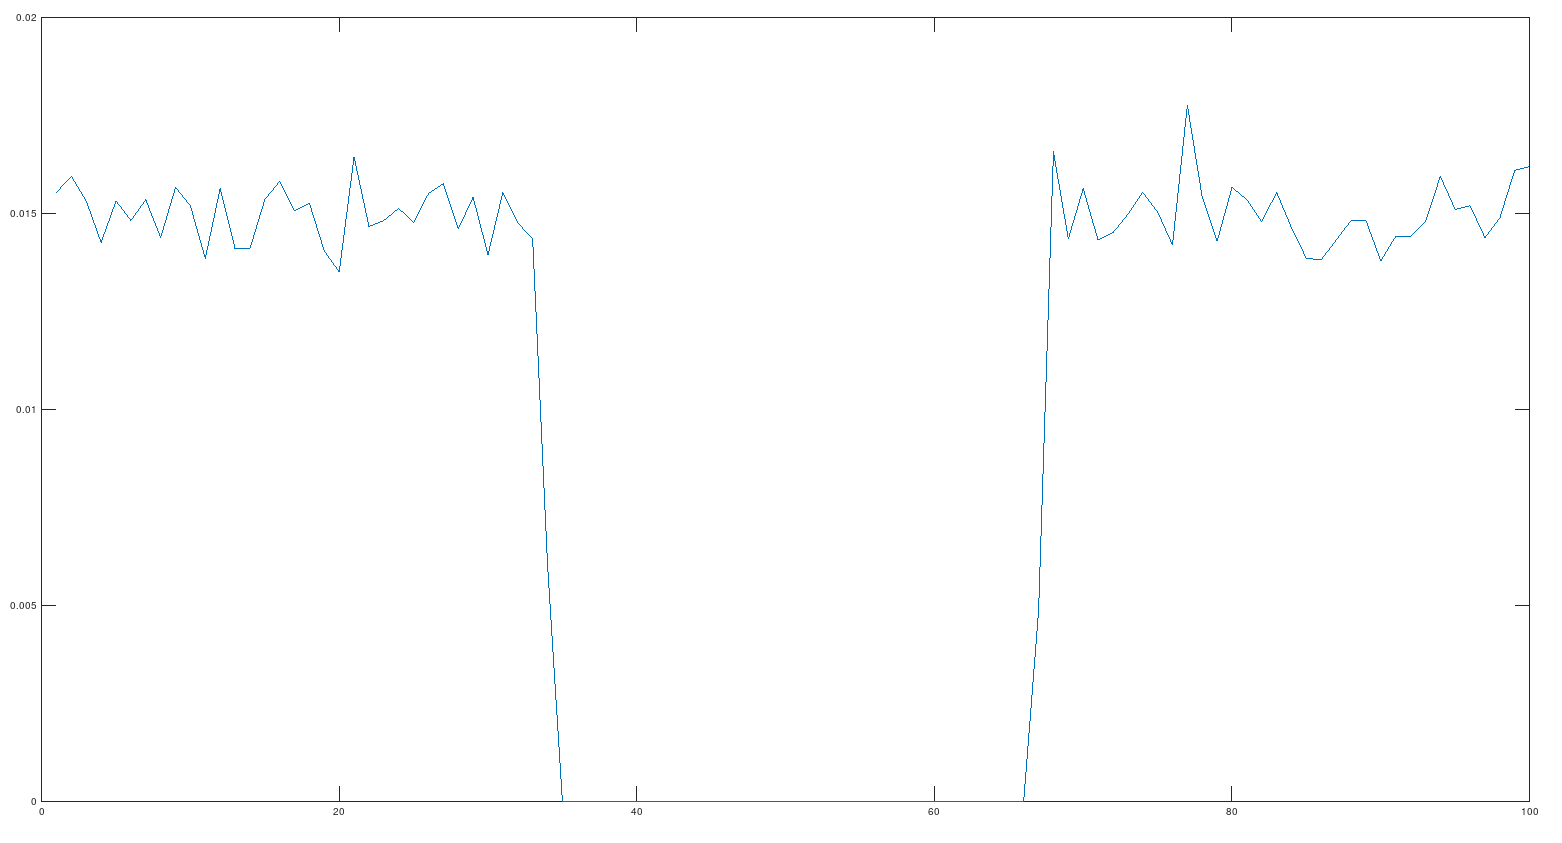
\includegraphics[width=\linewidth]{9}
\section{}
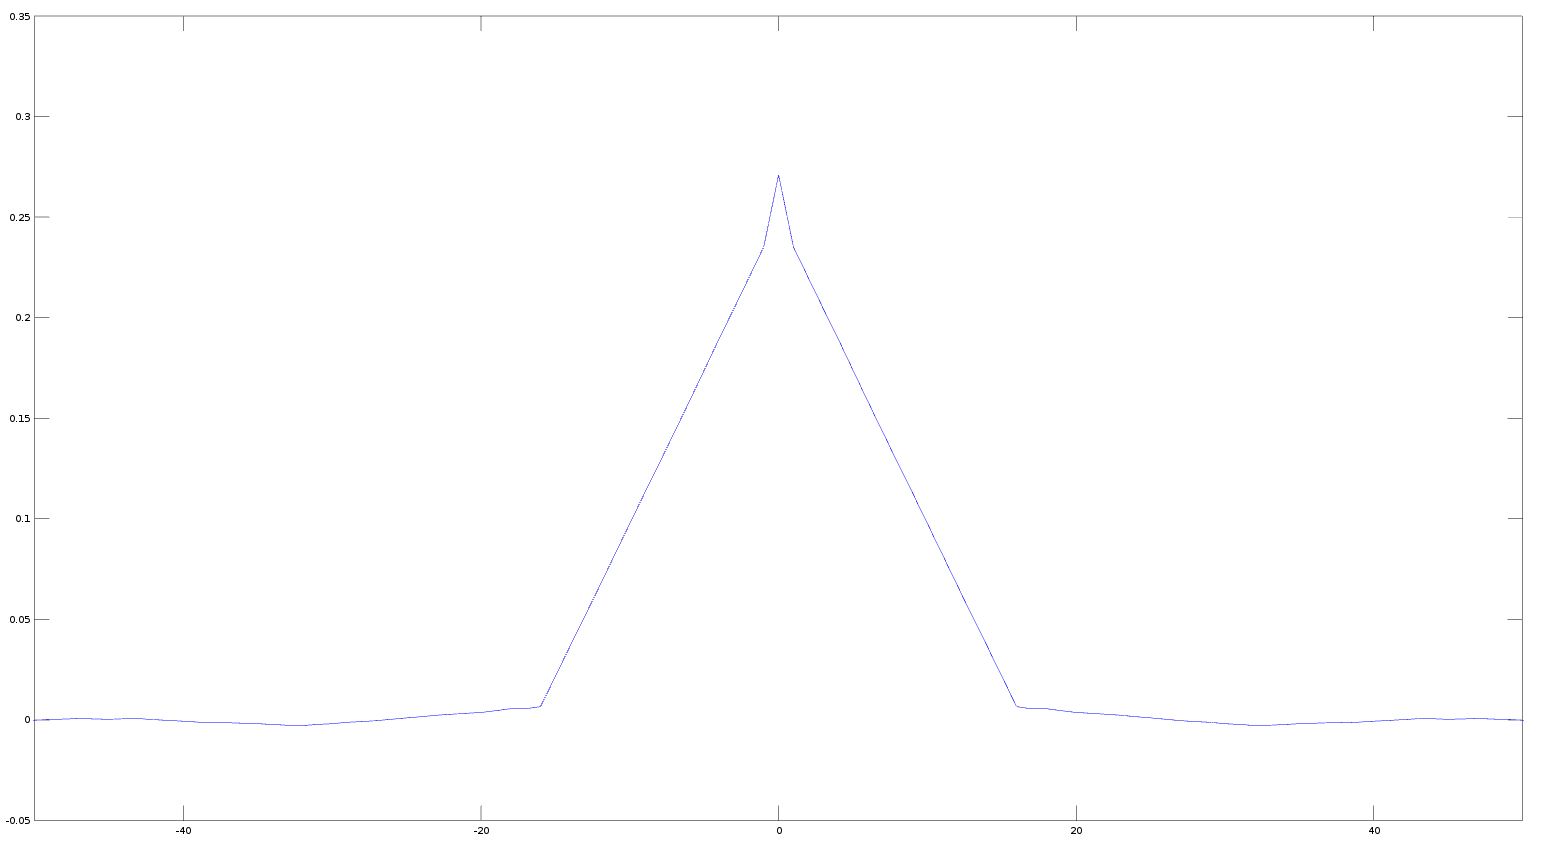
\includegraphics[width=\linewidth]{10}
\section{}
$R[0] = 0.27099 \\
R[1] = 0.097618 \\
R[16] = 0.0065915$
\section{}
Využil som funkciu hist2 a funkciu plot3.
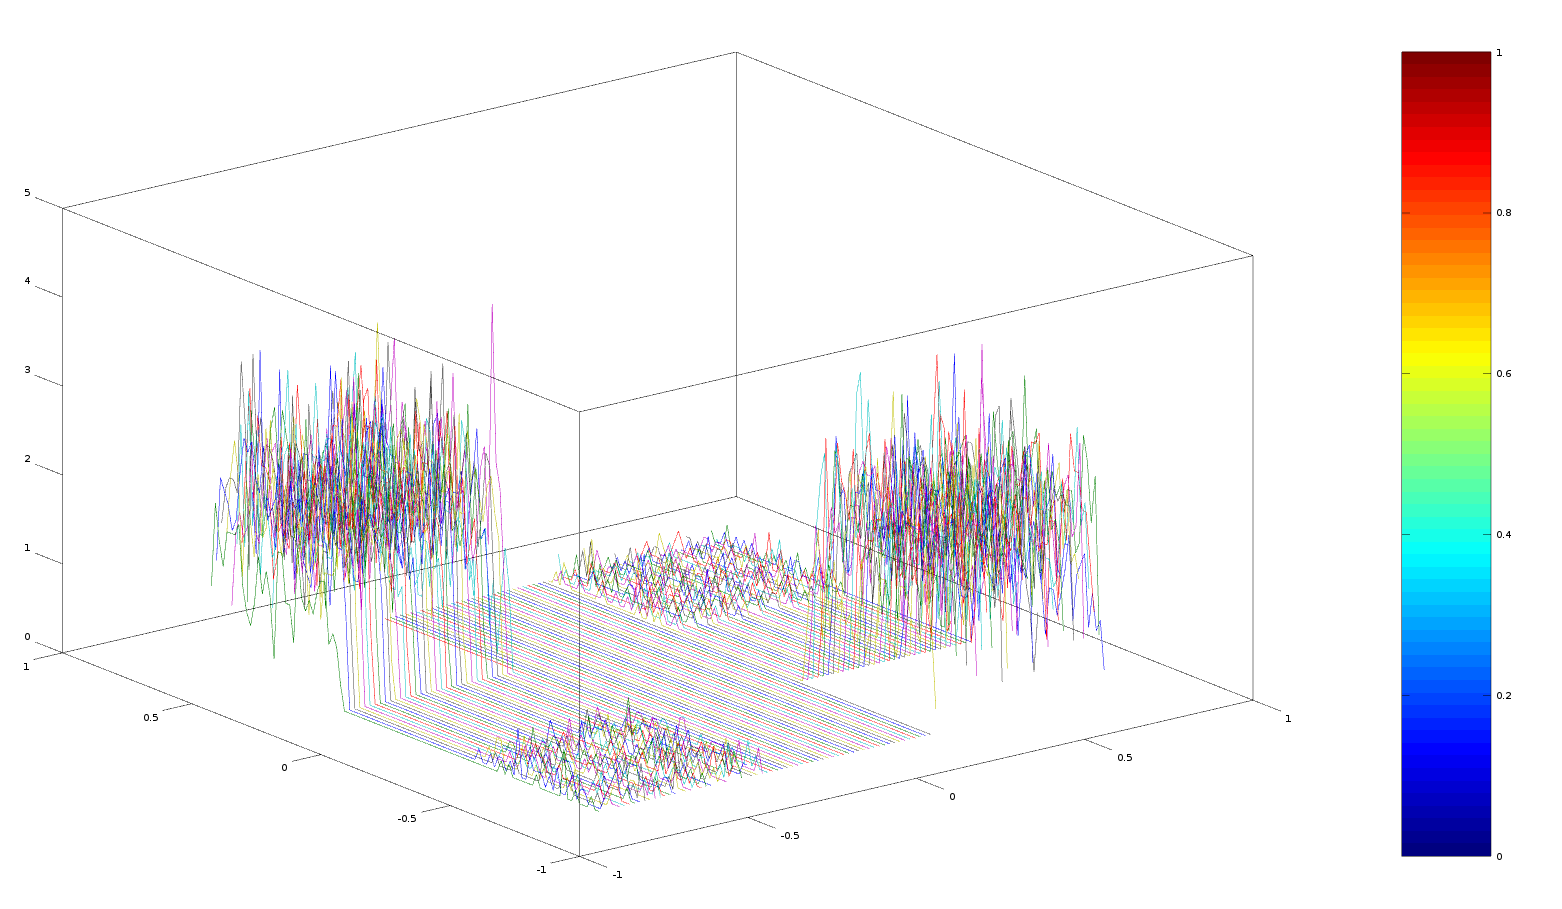
\includegraphics[width=\linewidth]{12}
\section{}
hist2: check -- 2d integral should be 1 and is 1
\section{}
Výsledok funkcie hist2 je 0.235146 a R1 z úlohy 10. je 0.23513. S prijateľnou odchýlkou po zaokrúhlení sú tieto hodnoty rovnaké.
\end{document}
